\section{Speech Recognition \& Audio Detection Test}

This test is divided in two phases. First the robot must answer a set of questions to an operator at the first attempt without asking for confirmation. The operator is not allowed to move to the robot or shout to the robot.

For the second phase, the focus is to carry out Sound Source Localization (SSL) and Automatic Speech Recognition (ASR) at the same time. To this effect, volunteers will stand around the robot and a randomly chosen volunteer will ask a question. The robot is expected to turn towards that volunteer and answer the question. If the robot is NOT able to carry out SSL and ASR at the same time (e.g. it needs to turn towards the speaking volunteer using SSL before doing ASR), the robot is allowed to request to repeat the question (with a penalty). In addition, if SSL cannot be carried out, the robot may still answer the question without turning, but no points will be provided for SSL.

\subsection{Goal}
The robot must be able to properly recognize and answer to a specific set of questions without ask for confirmation. Also, the robot shall be able to react to a speaking operator which is not facing towards to.

\subsection{Focus}

This test focuses on voice recognition and audio-source localization in a noisy environment, with moving sound sources\footnote{This test may also be held outside the arena}.

\subsection{Setup}
\begin{enumerate}
\item The apartment is in its normal state.
\item All doors of the apartment are open, except for the entry door. 
\end{enumerate}

\subsection{Task}

\begin{enumerate}
\item \textbf{Direct speech recognition: } The robot should move (or be moved) to a previously specified point inside the arena. 
  A TC member will ask 5 questions from the set of 50 predefined questions in front of the robot. 
  The robot should answer the question without asking confirmation.
  A question will only be asked once; there are no repetitions of a question. 
\begin{itemize}
\item The operator shall be standing still and facing to the robot.
\item The operator shall be between 0.75 and 1.0 meters away from the robot position.
\item The operator shall be between -60$^{\circ}$ and 60$^{\circ}$ from the robot's center (front range).
\end{itemize}
\item \textbf{Indirect speech recognition: } A group of several volunteers will stand around the robot as in Figure \ref{fig:asrsetup}, standing still, facing the robot, and between 0.75 to 1.0 meters away from it. The number of volunteers may change from the Figure. A random person of this group will ask a question of the same set described in the first part of the test. Before answering, the robot can do one or both of the following (each providing different amount of points):
\begin{itemize}
\item Answer the question,
\item Turn towards the person that asked the question,
\item Ask for only one repetition of the question, if needed (penalty).
\end{itemize}
This process will repeat 5 times. No attempt may receive negative points. When the robot provides an answer it should not ask for confirmation.
\end{enumerate}

\subsubsection{Questions}
% In previous years, the robots only had to answer questions from a list of pre-defined trivia questions. 
In addition to 10 predefined trivia-questions, the robot will be asked some questions about the RoboCup arena and the objects within it, i.e. the scenario. 

The questions will be about the colour, shape, size and type of the scenario objects \refsec{rule:scenario_objects} and where each object is usually found. 
For example:
\begin{itemize}
 \item What color is the shampoo? $\rightarrow$ The shampoo is blue.
 \item What is the color of the sponge $\rightarrow$ The sponge is green.
 \item What type of thing is the beer? $\rightarrow$ Beer a kind of drink. 
 \item Where can I find the beer? $\rightarrow$ The beer is in the fridge, nice and cool. 
 \item Tell me where the plates are. $\rightarrow$ The plate is in the cupboard. 
 \item How big is the egg? $\rightarrow$ The egg is a couple of centimeters big.
 \item What shape is the egg? $\rightarrow$ It is egg-shaped of course. 
 \item What shape is the soap? $\rightarrow$ The soap is a flat block. 
 \item Where is the shampoo? $\rightarrow$ The shampoo is in the closet. 
 \item What objects are in the closet? $\rightarrow$ The shampoo, soap, the sponge and a cloth. \textbf{Or:} The closet contains toiletries.
\end{itemize}
Note theat the robot does not have to go and find out the answer; it should be able to infer the answers from knowledge it already has. 

\begin{figure}[!h]
	\centering
	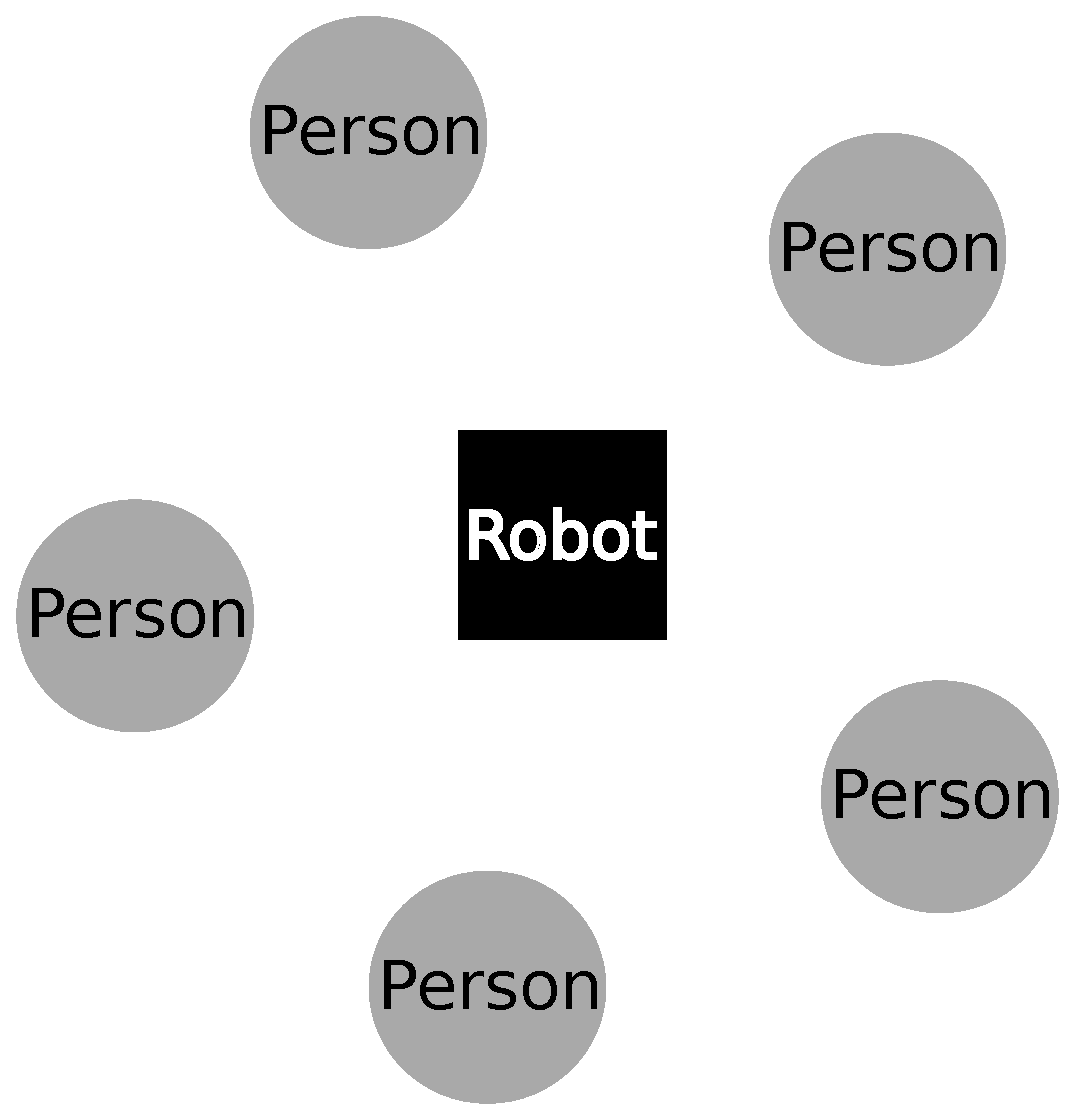
\includegraphics[width=0.5\columnwidth]{images/asrsetup.pdf}
	\caption{Speech recognition test: person setup around the robot for 2nd part.}
	\label{fig:asrsetup}
\end{figure}



\subsection{Additional rules and remarks}

\begin{itemize}
\item \textbf{Continue rule:} Continue rule (Section \refsec{rule:asrcontinue}) can not be used during this test.
\item \textbf{Question timeout:} If the robot does not answer within 10 seconds, the question is considered as \textit{missed}, and the TC member will proceed with the next question.
\item \textbf{Understanding the answer:} If the robot's answer is not understood by the operator, it is considered as \textit{incorrect}, and the TC member will proceed with the next question. It is thus advised that the robot provide answers such that it is clear that the robot understood the question. For example, if the question is ``What is the capital of Germany?'', instead of just answering ``Berlin'', it is advised that the robot answers something to the effect of ``The capital of Germany is Berlin''.
\item \textbf{Question repetition:} In the second phase, if the robot turns towards the operator to be asked once again, it should clearly state that it requires a repetition of the question once it finishes turning, so as to cue the operator to do so.
\end{itemize}

\subsection{Data recording}
  Please record the following data (See \refsec{rule:datarecording}):
  \begin{itemize}
   \item Audio
   \item Commands
  \end{itemize}

\subsection{Referee instructions}

The referee needs to
\begin{itemize}
\item Avoid shouting to the robot.
\item Avoid getting closer to the robot.
\item Speak to the robot loud and clear with plain standard English.
\item Avoid repeating questions for the same robot.
\item Choose the volunteers for the second part of the test, and describe this requirements to them.
\end{itemize}

\subsection{OC instructions}

\textbf{1 day before the test}
\begin{itemize}
\item Provide the set of 10 predefined questions
\item Prepare a set of questions about the RoboCup scenario. 
\end{itemize}
\textbf{2 hours before the test}
\begin{itemize}
\item Announce the placement of the robots
\end{itemize}

\subsection{Score sheet}
The maximum time for this test is 5 minutes.

\begin{scorelist}

	\scoreheading{Operator within the \textit{front range}}
	\scoreitem{10}{Correctly answered question 1}
	\scoreitem{10}{Correctly answered question 2}
	\scoreitem{10}{Correctly answered question 3}
	\scoreitem{10}{Correctly answered question 4}
	\scoreitem{10}{Correctly answered question 5}

	\scoreheading{Operator outside the \textit{front range}
	\footnotesize $2^{nd}$ attempt after asking operator to repeat the question}
	\scoreitem{20}{Correctly answered question 1 ($1^{st}$ attempt)}
	\scoreitem{10}{Correctly answered question 1 ($2^{nd}$ attempt)}
	\scoreitem{20}{Correctly answered question 2 ($1^{st}$ attempt)}
	\scoreitem{10}{Correctly answered question 2 ($2^{nd}$ attempt)}
	\scoreitem{20}{Correctly answered question 3 ($1^{st}$ attempt)}
	\scoreitem{10}{Correctly answered question 3 ($2^{nd}$ attempt)}
	\scoreitem{20}{Correctly answered question 4 ($1^{st}$ attempt)}
	\scoreitem{10}{Correctly answered question 4 ($2^{nd}$ attempt)}
	\scoreitem{20}{Correctly answered question 5 ($1^{st}$ attempt)}
	\scoreitem{10}{Correctly answered question 5 ($2^{nd}$ attempt)}

	\setTotalScore{150}
\end{scorelist}

% Local Variables:
% TeX-master: "Rulebook"
% End:


% Local Variables:
% TeX-master: "Rulebook"
% End:
